\PassOptionsToPackage{table}{xcolor}
\documentclass{beamer}
\usepackage{graphicx}
\usepackage{tikz}
\usepackage{enumerate}
\usepackage{xstring}
\usepackage{tcolorbox}
\usepackage{colortbl}
\tcbuselibrary{skins}

\usetikzlibrary{fit, positioning, shapes.geometric, arrows, shadows, calc, trees}


\usetheme{Madrid}
\usecolortheme{spruce}


\definecolor{myorange}{rgb}{0.85, 0.49, 0.13}
\definecolor{myblue}{rgb}{0.15, 0.65, 0.90}
\definecolor{mygreen}{rgb}{0.19, 0.82, 0.28}
\definecolor{myred}{rgb}{0.85, 0.11, 0.11}
\definecolor{mypurple}{rgb}{0.58, 0.29, 0.83}
\definecolor{myteal}{rgb}{0.19, 0.69, 0.63}
\definecolor{myyellow}{rgb}{0.95, 0.75, 0.15}
\definecolor{mybrown}{rgb}{0.65, 0.42, 0.20}
\definecolor{mydarkblue}{rgb}{0.2, 0.2, 0.6}
\definecolor{step1}{RGB}{255, 230, 153}
\definecolor{step2}{RGB}{189, 215, 238}
\definecolor{step3}{RGB}{197, 224, 180}
\definecolor{step4}{RGB}{244, 177, 131}
\definecolor{highlight}{RGB}{255, 242, 204}

\definecolor{buetgreen}{rgb}{0.0, 0.4, 0.2}
\definecolor{darkcharcoal}{rgb}{0.2, 0.2, 0.2}

\tcbset{
    refinedtitle/.style={
        colback=white,
        colframe=buetgreen,
        arc=3pt,
        boxrule=1.5pt,
        shadow={2pt}{-2pt}{0pt}{black!10},
        halign=center,
        width=0.95\textwidth
    }
}


\title{Hierarchical Clustering}
\subtitle{Building a Family Tree for Your Data}
\author{Group 7}
\institute{BUET CSE}

\begin{document}


\begin{frame}
    \begin{center}
        
        \vspace{0.2cm}

        
        
\begin{tikzpicture}[scale=0.5]
            \draw[buetgreen, thick] (0,1.5) -- (-1,0);
            \draw[buetgreen, thick] (0,1.5) -- (1,0);
            \filldraw[buetgreen] (0,1.5) circle (5pt);
            \filldraw[buetgreen!60] (-1,0) circle (4pt);
            \filldraw[buetgreen!60] (1,0) circle (4pt);
            \node[below, buetgreen!80, font=\Large\bfseries] at (0,-0.5) {Group 7};
        \end{tikzpicture}

        \vspace{0.4cm}

        
        \begin{tcolorbox}[refinedtitle]
            {\Huge \textbf{\textcolor{buetgreen}{Hierarchical Clustering}}} \\
            \vspace{0.2cm}
            {\large \textit{\textcolor{darkcharcoal}{Building a Family Tree for Your Data}}}
        \end{tcolorbox}

        \vspace{0.6cm}

        
        \begin{columns}[t]
            \column{0.33\textwidth}
            \centering
            \textbf{\small Apurbo Das Pranto}\\
            \scriptsize ID: 2205091
            
            \column{0.33\textwidth}
            \centering
            \textbf{\small Mahrez Hussain Khan}\\
            \scriptsize ID: 2205109
            
            \column{0.33\textwidth}
            \centering
            \textbf{\small Md. Tanveer Hossain}\\
            \scriptsize ID: 2205112
        \end{columns}

        \vfill

        
        
\begin{tikzpicture}
            \draw[buetgreen!40, thick] (0,0) -- (3,0);
        \end{tikzpicture}
        
        \vspace{0.1cm}
        {\small \textbf{Department of Computer Science and Engineering}} \\
        {\footnotesize Bangladesh University of Engineering and Technology} \\
        \vspace{0.2cm}
        {\scriptsize \today}
        
    \end{center}
\end{frame}

\begin{frame}{Outline}
    \tableofcontents
\end{frame}


\section{Introduction - Clustering Basics}


\begin{frame}{A Problem to Think About}

\begin{example}[Superstore Customer Problem]
A large superstore wants to understand their 10,000 customers better. They have data about each customer:
\begin{itemize}
    \item<2-> \textbf{Age} (25, 30, 45, 50, etc.)
    \item<3-> \textbf{Monthly Expense} (\$100, \$500, \$1000, etc.)
    \item<4-> \textbf{Shopping Preferences} (Electronics, Grocery, Fashion, etc.)
\end{itemize}
\end{example}

\vspace{0.2cm}

\only<5->{
\begin{alertblock}{The Question}
\textbf{How can they group these customers to create targeted offers for each group?}
\end{alertblock}
}

\only<1-4>{
\begin{center}
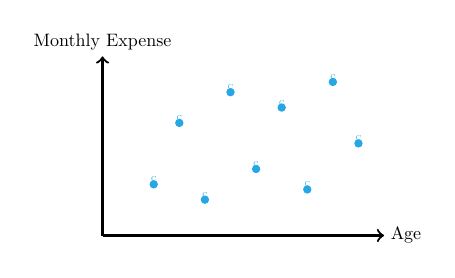
\begin{tikzpicture}[scale=0.65, transform shape]
    
    \draw[->, thick] (0,0) -- (5.5,0) node[right] {Age};
    \draw[->, thick] (0,0) -- (0,3.5) node[above] {Monthly Expense};
    
    
    \foreach \x/\y in {1/1.0, 1.5/2.2, 2/0.7, 2.5/2.8, 3/1.3, 3.5/2.5, 4/0.9, 4.5/3.0, 5/1.8} {
        \filldraw[myblue] (\x,\y) circle (2pt) node[above, scale=0.4] {C};
    }
\end{tikzpicture}
\end{center}
}

\only<6>{
\begin{tcolorbox}[colback=myblue!5, colframe=myblue, title=Think, width=\textwidth]
\centering
\Large
Manually grouping 10,000 customers? \textcolor{myred}{Impossible!}
\end{tcolorbox}
}

\end{frame}


\begin{frame}{Solution: Clustering!}

\begin{columns}[T]
    \column{0.4\textwidth}
    \begin{itemize}
        \item<1-> \textbf{Clustering} automatically groups similar customers
        \item<5-> Each group = \textcolor{myorange}{Cluster}
        \item<6-> Boundaries define each cluster with \textbf{meaningful names}
        \item<7-> Customers in same cluster have similar:
            \begin{itemize}
                \item Age
                \item Spending habits
                \item Preferences
            \end{itemize}
    \end{itemize}
    
    \column{0.6\textwidth}
    \begin{center}
        \begin{tikzpicture}[scale=0.8, transform shape]
            
            \draw[->, thick, black!90] (0,0) -- (7.0,0) node[right] {Age};
            \draw[->, thick, black!90] (0,0) -- (0,5.5) node[above] {Monthly Expense};
            
            
            \draw[very thin, black!40] (0,0) grid (7.0,5.5);
            
           
            \only<1-4>{
                
                \filldraw[black!60] (1.8,4.2) circle (4pt);
                \filldraw[black!60] (2.8,4.7) circle (4pt);
                \filldraw[black!60] (3.5,4.5) circle (4pt);
                \filldraw[black!60] (2.2,5.0) circle (4pt);
                \filldraw[black!60] (1.2,4.8) circle (4pt);
                
                
                \filldraw[black!60] (4.2,2.2) circle (4pt);
                \filldraw[black!60] (5.2,2.5) circle (4pt);
                \filldraw[black!60] (4.8,3.2) circle (4pt);
                \filldraw[black!60] (5.8,2.7) circle (4pt);
                \filldraw[black!60] (3.8,2.9) circle (4pt);
                
                
                \filldraw[black!60] (1.2,0.9) circle (4pt);
                \filldraw[black!60] (2.0,1.1) circle (4pt);
                \filldraw[black!60] (1.6,1.8) circle (4pt);
                \filldraw[black!60] (2.5,0.8) circle (4pt);
            }
            
            
            \only<2>{
                
                \filldraw[myblue!90] (1.8,4.2) circle (5pt);
                \filldraw[myblue!90] (2.8,4.7) circle (5pt);
                \filldraw[myblue!90] (3.5,4.5) circle (5pt);
                \filldraw[myblue!90] (2.2,5.0) circle (5pt);
                \filldraw[myblue!90] (1.2,4.8) circle (5pt);
                
                
                \draw[myblue!90, line width=1.2pt] (1.8,4.2) -- (2.8,4.7);
                \draw[myblue!90, line width=1.2pt] (2.8,4.7) -- (3.5,4.5);
                \draw[myblue!90, line width=1.2pt] (3.5,4.5) -- (2.2,5.0);
                \draw[myblue!90, line width=1.2pt] (2.2,5.0) -- (1.2,4.8);
                \draw[myblue!90, line width=1.2pt] (1.2,4.8) -- (1.8,4.2);
                
                
                \filldraw[black!60] (4.2,2.2) circle (4pt);
                \filldraw[black!60] (5.2,2.5) circle (4pt);
                \filldraw[black!60] (4.8,3.2) circle (4pt);
                \filldraw[black!60] (5.8,2.7) circle (4pt);
                \filldraw[black!60] (3.8,2.9) circle (4pt);
                \filldraw[black!60] (1.2,0.9) circle (4pt);
                \filldraw[black!60] (2.0,1.1) circle (4pt);
                \filldraw[black!60] (1.6,1.8) circle (4pt);
                \filldraw[black!60] (2.5,0.8) circle (4pt);
            }
            
            
            \only<3>{
                
                \filldraw[mygreen!90] (4.2,2.2) circle (5pt);
                \filldraw[mygreen!90] (5.2,2.5) circle (5pt);
                \filldraw[mygreen!90] (4.8,3.2) circle (5pt);
                \filldraw[mygreen!90] (5.8,2.7) circle (5pt);
                \filldraw[mygreen!90] (3.8,2.9) circle (5pt);
                
                
                \draw[mygreen!90, line width=1.2pt] (4.2,2.2) -- (5.2,2.5);
                \draw[mygreen!90, line width=1.2pt] (5.2,2.5) -- (5.8,2.7);
                \draw[mygreen!90, line width=1.2pt] (5.8,2.7) -- (4.8,3.2);
                \draw[mygreen!90, line width=1.2pt] (4.8,3.2) -- (3.8,2.9);
                \draw[mygreen!90, line width=1.2pt] (3.8,2.9) -- (4.2,2.2);
                
                
                \filldraw[myblue!90] (1.8,4.2) circle (5pt);
                \filldraw[myblue!90] (2.8,4.7) circle (5pt);
                \filldraw[myblue!90] (3.5,4.5) circle (5pt);
                \filldraw[myblue!90] (2.2,5.0) circle (5pt);
                \filldraw[myblue!90] (1.2,4.8) circle (5pt);
                
                
                \filldraw[black!60] (1.2,0.9) circle (4pt);
                \filldraw[black!60] (2.0,1.1) circle (4pt);
                \filldraw[black!60] (1.6,1.8) circle (4pt);
                \filldraw[black!60] (2.5,0.8) circle (4pt);
            }
            
            
            \only<4>{
               
                \filldraw[myred!90] (1.2,0.9) circle (5pt);
                \filldraw[myred!90] (2.0,1.1) circle (5pt);
                \filldraw[myred!90] (1.6,1.8) circle (5pt);
                \filldraw[myred!90] (2.5,0.8) circle (5pt);
                
                
                \draw[myred!90, line width=1.2pt] (1.2,0.9) -- (2.0,1.1);
                \draw[myred!90, line width=1.2pt] (2.0,1.1) -- (2.5,0.8);
                \draw[myred!90, line width=1.2pt] (2.5,0.8) -- (1.6,1.8);
                \draw[myred!90, line width=1.2pt] (1.6,1.8) -- (1.2,0.9);
                
                
                \filldraw[myblue!90] (1.8,4.2) circle (5pt);
                \filldraw[myblue!90] (2.8,4.7) circle (5pt);
                \filldraw[myblue!90] (3.5,4.5) circle (5pt);
                \filldraw[myblue!90] (2.2,5.0) circle (5pt);
                \filldraw[myblue!90] (1.2,4.8) circle (5pt);
                
                \filldraw[mygreen!90] (4.2,2.2) circle (5pt);
                \filldraw[mygreen!90] (5.2,2.5) circle (5pt);
                \filldraw[mygreen!90] (4.8,3.2) circle (5pt);
                \filldraw[mygreen!90] (5.8,2.7) circle (5pt);
                \filldraw[mygreen!90] (3.8,2.9) circle (5pt);
            }
            
        
            \only<5->{
                
                \filldraw[myred!90] (1.2,0.9) circle (5pt);
                \filldraw[myred!90] (2.0,1.1) circle (5pt);
                \filldraw[myred!90] (1.6,1.8) circle (5pt);
                \filldraw[myred!90] (2.5,0.8) circle (5pt);
                
                \filldraw[mygreen!90] (4.2,2.2) circle (5pt);
                \filldraw[mygreen!90] (5.2,2.5) circle (5pt);
                \filldraw[mygreen!90] (4.8,3.2) circle (5pt);
                \filldraw[mygreen!90] (5.8,2.7) circle (5pt);
                \filldraw[mygreen!90] (3.8,2.9) circle (5pt);
                
                \filldraw[myblue!90] (1.8,4.2) circle (5pt);
                \filldraw[myblue!90] (2.8,4.7) circle (5pt);
                \filldraw[myblue!90] (3.5,4.5) circle (5pt);
                \filldraw[myblue!90] (2.2,5.0) circle (5pt);
                \filldraw[myblue!90] (1.2,4.8) circle (5pt);
                
                
                \draw[myred!90, dashed, very thick] (1.9,1.2) ellipse (1.2cm and 0.8cm);
                \node[myred!90, font=\bfseries\large, scale=0.8] at (1.9,0.0) {STUDENTS};
                
                \draw[mygreen!90, dashed, very thick] (4.8,2.7) ellipse (1.3cm and 0.8cm);
                \node[mygreen!90, font=\bfseries\large, scale=0.8] at (4.8,1.5) {FAMILIES};
                
                \draw[myblue!90, dashed, very thick] (2.3,4.7) ellipse (1.3cm and 0.8cm);
                
                \node[myblue!90, font=\bfseries\large, scale=0.8] at (2.3,5.9) {PREMIUM};
            }
        \end{tikzpicture}
    \end{center}
\end{columns}

\vfill
\only<7->{
\begin{exampleblock}{}
\centering
\large
\textbf{Each cluster contains customers with similar characteristics!}
\end{exampleblock}
}
\end{frame}


\begin{frame}{What is Clustering?}

\begin{columns}[T]
    \column{0.50\textwidth}
    \begin{block}{Definition}
        \centering
        \large
        \textbf{Clustering} is the process of \\
        \textbf{\textcolor{myorange}{dividing the datasets}} into groups, \\
        consisting of \textbf{\textcolor{myorange}{similar data-points}}.
    \end{block}
    
    \vspace{0.3cm}
    
    \begin{block}{Analogy}
        \centering
        \large
        Like sorting a fruit basket: all \\
        \textbf{\textcolor{myred}{apples}} go in one bowl, all \textbf{\textcolor{mygreen}{oranges}} \\
        in another.
    \end{block}
    
    \column{0.52\textwidth}
    \begin{center}
        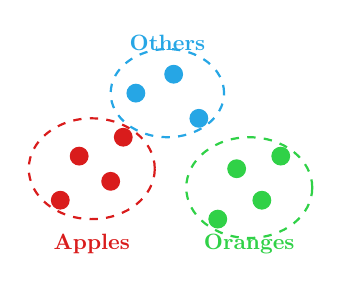
\begin{tikzpicture}[scale=0.8, transform shape]
           
            \filldraw[myred] (1.0,1.5) circle (4pt);
            \filldraw[myred] (1.8,1.8) circle (4pt);
            \filldraw[myred] (1.3,2.2) circle (4pt);
            \filldraw[myred] (2.0,2.5) circle (4pt);
            \draw[myred, dashed, thick] (1.5,2.0) ellipse (1.0cm and 0.8cm);
            \node[myred, font=\bfseries] at (1.5,0.8) {Apples};
            
            
            \filldraw[mygreen] (3.5,1.2) circle (4pt);
            \filldraw[mygreen] (4.2,1.5) circle (4pt);
            \filldraw[mygreen] (3.8,2.0) circle (4pt);
            \filldraw[mygreen] (4.5,2.2) circle (4pt);
            \draw[mygreen, dashed, thick] (4.0,1.7) ellipse (1.0cm and 0.8cm);
            \node[mygreen, font=\bfseries] at (4.0,0.8) {Oranges};
            
            
            \filldraw[myblue] (2.2,3.2) circle (4pt);
            \filldraw[myblue] (2.8,3.5) circle (4pt);
            \filldraw[myblue] (3.2,2.8) circle (4pt);
            \draw[myblue, dashed, thick] (2.7,3.2) ellipse (0.9cm and 0.7cm);
            \node[myblue, font=\bfseries] at (2.7,4.0) {Others};
        \end{tikzpicture}
    \end{center}
\end{columns}

\end{frame}


\section{Transition to Hierarchical Clustering}


\begin{frame}{What's Missing?}
\begin{center}
    \vspace{0.5cm}
    
    \begin{tcolorbox}[colback=myorange!20, colframe=myorange, width=0.8\textwidth, rounded corners]
        \centering
        \Huge \textbf{But...}
    \end{tcolorbox}
    
    \onslide<2->{
    \begin{block}{}
        \centering
        \Large
        Regular clustering gives us \textbf{groups}...
    \end{block}
    }
    
    \vspace{0.3cm}
    
    \onslide<3->{
    \begin{block}{}
        \centering
        \Large
        But it doesn't tell us \textbf{\textcolor{myorange}{how groups are related}} to each other!
    \end{block}
    }
    
    \vspace{0.3cm}
    
    \onslide<4->{
    \begin{alertblock}{}
        \centering
        \LARGE
        \textbf{We need \textcolor{myorange}{something more}...}
    \end{alertblock}
    }
    
\end{center}
\end{frame}


\begin{frame}{}
\begin{center}
    \vspace{0.5cm}
    
    \begin{tcolorbox}[colback=mygreen!20, colframe=mygreen, width=0.7\textwidth, rounded corners]
        \centering
        \Huge \textbf{Here Comes...}
    \end{tcolorbox}
    
    \vspace{0.5cm}
    
    
    \begin{center}
        
\includegraphics[width=0.45\textwidth]{images/thor.jpg}
    \end{center}
    
    \vspace{0.3cm}
    
    \begin{tcolorbox}[colback=myblue!20, colframe=myblue, width=0.8\textwidth]
        \centering
        \LARGE \textbf{\textcolor{myorange}{Hierarchical Clustering!}}
    \end{tcolorbox}
    
\end{center}
\end{frame}


\begin{frame}{}
\begin{center}
    \vspace{0.5cm}
    
    \begin{tcolorbox}[colback=myblue!10, colframe=myblue, width=0.7\textwidth]
        \centering
        \Huge \textbf{ DONE! }
    \end{tcolorbox}
    
    \vspace{0.4cm}
    
    \begin{block}{\textcolor{myorange}{\textbf{What we covered? } }}
    \centering
    \large
        \item \textcolor{myblue}{\textbf{Real-life Problem Example}}
                \item \textcolor{myblue}{\textbf{Clustering Fundamentals}}
        \item \textcolor{myblue}{\textbf{The Need of Hierarchical Clustering}}

    \end{block}
    
    \vspace{0.4cm}
    
\begin{tcolorbox}[colback=myorange!10, colframe=myorange, width=0.8\textwidth]
    \centering
    \Large
    \textbf{ Over to \textcolor{myorange}{Speaker 2} }
\end{tcolorbox}
    
\end{center}
\end{frame}


\section{Hierarchical Clustering - Introduction}

\begin{frame}{Definition of Hierarchical Clustering}
    \pause
    \begin{block}{Hierarchical Clustering}
        \textbf{\textbf{Hierarchical cluster analysis}} or \textbf{HCA} is a method of cluster analysis that builds a \textbf{tree structure} (\textit{dendrogram}) from data similarities.
    \end{block}

\end{frame}


\begin{frame}{Dendrogram}
    \centering
    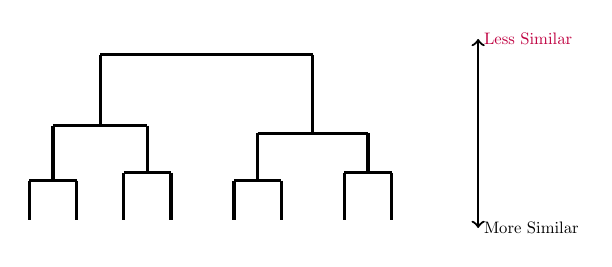
\begin{tikzpicture}
            
            \draw[black,very thick] (0.8,0.6) -- (1.4,0.6);
            \draw[black,very thick] (0.8,0.6) -- (0.8,0.1);
            \draw[black,very thick] (1.4,0.6) -- (1.4,0.1);

            \draw[black,very thick] (2.0,0.7) -- (2.6,0.7);
            \draw[black,very thick] (2.0,0.7) -- (2.0,0.1);
            \draw[black,very thick] (2.6,0.7) -- (2.6,0.1);

            
            \draw[black,very thick] (3.4,0.6) -- (4.0,0.6);
            \draw[black,very thick] (3.4,0.6) -- (3.4,0.1);
            \draw[black,very thick] (4.0,0.6) -- (4.0,0.1);

            
            \draw[black,very thick] (4.8,0.7) -- (5.4,0.7);
            \draw[black,very thick] (4.8,0.7) -- (4.8,0.1);
            \draw[black,very thick] (5.4,0.7) -- (5.4,0.1);

            
            \draw[black,very thick] (1.1,1.3) -- (2.3,1.3);
            \draw[black,very thick] (1.1,1.3) -- (1.1,0.6);
            \draw[black,very thick] (2.3,1.3) -- (2.3,0.7);

            
            \draw[black,very thick] (3.7,1.2) -- (5.1,1.2);
            \draw[black,very thick] (3.7,1.2) -- (3.7,0.6);
            \draw[black,very thick] (5.1,1.2) -- (5.1,0.7);

            \draw[black,very thick] (1.7,2.2) -- (4.4,2.2);
            \draw[black,very thick] (1.7,2.2) -- (1.7,1.3);
            \draw[black,very thick] (4.4,2.2) -- (4.4,1.2);

            \draw[<->,thick] (6.5,0) -- (6.5,2.4);
            \node[purple,right,scale=0.6] at (6.5,2.4) {Less Similar};
            \node[black,right,scale=0.6] at (6.5,0) {More Similar};
            
        \end{tikzpicture}

\end{frame}

\section{Types of Hierarchical Clustering}
\begin{frame}{Types of Hierarchical Clustering}
    \pause
    \begin{block}{Agglomerative}
        Bottom-Up Approach\pause
    \end{block}
    \begin{block}{Divisive}
        Top-Down Approach
    \end{block}
\end{frame}
\subsection{Agglomerative Clustering}
\begin{frame}{Agglomerative Clustering (Bottom-Up)}
    \begin{columns}[c]
        \centering
        \column{0.48\textwidth}
            \begin{block}{Agglomerative (Bottom-Up)}
                \begin{enumerate}
                    \item<2-> Start with each point as its own cluster.
                    \item<3-> \textbf{Merge} the two \textcolor{myorange}{closest} clusters.
                    \item<4-> Repeat until one big cluster remains.
                \end{enumerate}
            \end{block}
        \centering
        \column{0.48\textwidth}
        \centering
        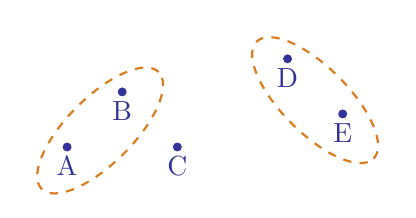
\begin{tikzpicture}[scale=0.7]
            \onslide<2->\filldraw[mydarkblue] (0,0) circle (2pt) node[below] {A};
            \onslide<2->\filldraw[mydarkblue] (1.0,1.0) circle (2pt) node[below] {B};
            \onslide<2->\filldraw[mydarkblue] (2,0) circle (2pt) node[below] {C};
            \onslide<2->\filldraw[mydarkblue] (4,1.6) circle (2pt) node[below] {D};
            \onslide<2->\filldraw[mydarkblue] (5.0,0.6) circle (2pt) node[below] {E};
            \onslide<3->{\draw[myorange, dashed, thick](0.6,0.3)ellipse [x radius=1.5cm, y radius=0.6cm,rotate=45];}
            \onslide<4->{\draw[myorange, dashed, thick](4.5,0.85)ellipse [x radius=1.5cm, y radius=0.6cm, rotate=-45];}
        \end{tikzpicture}

        \onslide<5->{\textbf{and so on...}}
        
    \end{columns}
    
\end{frame}
\begin{frame}{Agglomerative Clustering Example}
    \begin{columns}[c]
        \centering
        \column{0.5\textwidth}
        \begin{tikzpicture}[scale=0.12]
        
            \draw[thick] (15,20) rectangle (50,45);
            
            
            \foreach \x in {15,20,25,30,35,40,45,50}
                \node[below] at (\x,20) {\x};
            
            \foreach \y in {20,25,30,35,40,45}
                \node[left] at (15,\y) {\y};
            
            
            \draw[very thick, black, rotate around={25:(32,32)}]
            (32,32) ellipse (17 and 10);
            
            
            \draw[blue, thick, dashed, rotate around={30:(40,36)}]
            (40,36) ellipse (7 and 5);
            \only<22-25>\draw[very thick, rotate around={30:(40,36)}](40,36) ellipse (7 and 5);
            
            
            \draw[blue, thick, dashed, rotate around={30:(40,37)}]
            (40,37) ellipse (5 and 3);
            \only<18-20>\draw[very thick, rotate around={30:(40,37)}](40,37) ellipse (5 and 3);
            
            \node[blue, font=\tiny] at (43,33.6) {$P_1$};
            \onslide<17-20>{\draw[very thick] (43,33.6) circle (1.5cm);}
            
            \node[blue, font=\tiny] at (37.5,35.5) {$P_2$};
            \onslide<7-10>{\draw[very thick] (37.5,35.5) circle (1.5cm);}
            \node[blue, font=\tiny] at (42.5,39) {$P_3$};
            \onslide<8-10>{\draw[very thick] (42.5,39) circle (1.5cm);}
            
            
            \draw[green!60!black, thick, dashed, rotate around={-20:(24,27.7)}]
            (24,27) ellipse (7 and 6);
            \only<23-25>\draw[very thick, rotate around={-20:(24,27.7)}](24,27) ellipse (7 and 6);
            
            
            \draw[green!60!black, thick, dashed, rotate around={-20:(22.8,26)}](22.8,26) ellipse (5 and 4);
            \only<13-15>\draw[very thick, rotate around={-20:(22.8,26)}](22.8,26) ellipse (5 and 4);
            
            \node[green!60!black, font=\tiny] at (26.5,31) {$P_4$};
            \onslide<12-15>{\draw[very thick] (26.5,31) circle (1.5cm);}
            \node[green!60!black, font=\tiny] at (20,28) {$P_5$};
            \onslide<2-5>{\draw[very thick] (20,28) circle (1.5cm);}
            \node[green!60!black, font=\tiny] at (25,23.5) {$P_6$};
            \onslide<3-5>{\draw[very thick] (25,23.5) circle (1.5cm);}
            
        
        \end{tikzpicture}
        \centering
        \column{0.5\textwidth}
        \centering
        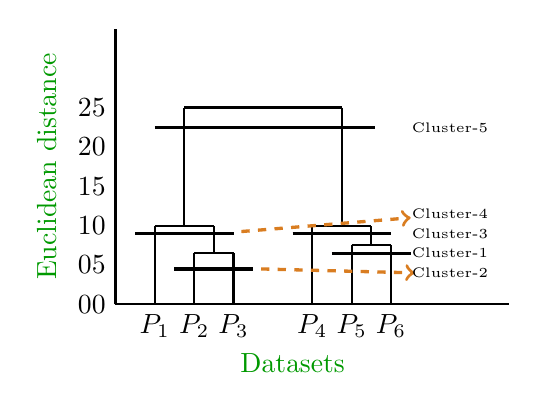
\begin{tikzpicture}[scale=0.5]
        
            
            \draw[thick] (0,0) -- (0,7);
            \draw[thick] (0,0) -- (10,0);
            
            
            \foreach \y/\label in {0/00,1/05,2/10,3/15,4/20,5/25}
                \node[left] at (0,\y) {\label};
            
            
            \node[rotate=90, green!60!black] at (-1.75,3.5) {Euclidean distance};
            \node[green!60!black] at (4.5,-1.5) {Datasets};

            
            
            
            \node at (1,0) [below] {$P_1$};
            \node at (2,0) [below] {$P_2$};
            \node at (3,0) [below] {$P_3$};
            \node at (5,0) [below] {$P_4$};
            \node at (6,0) [below] {$P_5$};
            \node at (7,0) [below] {$P_6$};
            
            
            \draw[thick] (1,0) -- (1,2);
            \draw[thick] (2,0) -- (2,1.3);
            \draw[thick] (3,0) -- (3,1.3);
            
            \draw[thick] (2,1.3) -- (3,1.3);
            \draw[thick] (2.5,1.3) -- (2.5,2);
            
            \draw[thick] (1,2) -- (2.5,2);
            
            
            \draw[thick] (5,0) -- (5,2);
            \draw[thick] (6,0) -- (6,1.5);
            \draw[thick] (7,0) -- (7,1.5);
            
            \draw[thick] (6,1.5) -- (7,1.5);
            \draw[thick] (6.5,1.5) -- (6.5,2);
            
            \draw[thick] (5,2) -- (6.5,2);
            
            
            \draw[thick] (1.75,5) -- (5.75,5);
            \draw[thick] (1.75,5) -- (1.75,2);
            \draw[thick] (5.75,5) -- (5.75,2);
            
            
            \onslide<14>{\draw[magenta, thick] (4.5,1.8) -- (7,1.8);}
            \onslide<15->{\draw[black, very thick] (4.5,1.8) -- (7,1.8);}
            \onslide<15->\node[black,font=\tiny] at (8.5,1.8) {Cluster-3};
            \onslide<19>{\draw[magenta, thick] (0.5,1.8) -- (3,1.8);}
            \onslide<20->{\draw[black, very thick] (0.5,1.8) -- (3,1.8);}
            \onslide<20->\node[black,font=\tiny] at (8.5,2.3) {Cluster-4};
            \onslide<20->\draw[myorange, dashed,very thick, ->] (3.2,1.85) -- (7.5,2.2);
            \onslide<24>{\draw[magenta, thick] (1,4.5) -- (6.6,4.5);}
            \onslide<25->{\draw[black, very thick] (1,4.5) -- (6.6,4.5);}
            \onslide<25->\node[black,font=\tiny] at (8.5,4.5) {Cluster-5};
           
            
            \onslide<9>\draw[magenta, thick] (1.5,0.9) -- (3.5,0.9);
            \onslide<10->\draw[black, very thick] (1.5,0.9) -- (3.5,0.9);
            \onslide<10->\draw[myorange, dashed,very thick, ->] (3.7,0.9) -- (7.6,.8);
            \onslide<10->\node[black,font=\tiny] at (8.5,.8) {Cluster-2};
            \onslide<4>\draw[magenta, thick] (5.5,1.3) -- (7.5,1.3);
            \onslide<5->\draw[black, very thick] (5.5,1.3) -- (7.5,1.3);
            \onslide<5->\node[black,font=\tiny] at (8.5,1.3) {Cluster-1};
        \end{tikzpicture}

    \end{columns}
\end{frame}
\subsection{Divisive Clustering}
\begin{frame}{Divisive Clustering}
    \begin{columns}[c]
        \centering
        \column{0.48\textwidth}
        \begin{block}{Divisive (Top-Down)}
            \begin{enumerate}
                \item<2-> Start with all points in one big cluster.
                \item<3-> \textbf{Split} a cluster into two smaller ones.
                \item<4-> Repeat until each point is its own cluster.
            \end{enumerate}
        \end{block}
        \centering
        \column{0.48\textwidth}
        \centering
        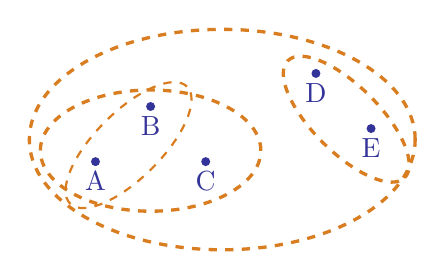
\begin{tikzpicture}[scale=0.7]
                \onslide<2>{\draw[myorange, dashed, very thick] (2.3,0.4) ellipse (3.5cm and 2cm);}
                \onslide<3>{\draw[myorange, dashed, very thick] (1,0.2) ellipse (2cm and 1.1cm);}
                \onslide<3->{\draw[myorange, dashed, very thick](4.55,0.77) ellipse [x radius=1.5cm, y radius=0.6cm,rotate=-45];}
                \onslide<4>{\draw[myorange, dashed, thick](0.6,0.3)ellipse [x radius=1.5cm, y radius=0.6cm,rotate=45];}
                \onslide<2->\filldraw[mydarkblue] (0,0) circle (2pt) node[below] {A};
                \onslide<2->\filldraw[mydarkblue] (1.0,1.0) circle (2pt) node[below] {B};
                \onslide<2->\filldraw[mydarkblue] (2,0) circle (2pt) node[below] {C};
                \onslide<2->\filldraw[mydarkblue] (4,1.6) circle (2pt) node[below] {D};
                \onslide<2->\filldraw[mydarkblue] (5.0,0.6) circle (2pt) node[below] {E};
        \end{tikzpicture}

        \onslide<4->{\textbf{and so on...}}
    \end{columns}
\end{frame}
\begin{frame}
    \centering
    \begin{tcolorbox}[colback=white, colframe=mygreen, title=Which is more common?]
        \textcolor{myorange}{Agglomerative} is more popular because it's computationally simpler.
    \end{tcolorbox}
\end{frame}
\section{Linkage Criteria}
\begin{frame}{How Do We Define ``Closeness''? (Linkage Methods)}
    \begin{columns}
        \column{0.5\textwidth}
            \begin{itemize}
                \item<1-> \textbf{Single Linkage (Min):}
                    \begin{itemize}
                        \item Closest pair of points.
                        \item \textit{Can lead to ``chaining'' (long, thin clusters).}
                    \end{itemize}
                \item<2-> \textbf{Complete Linkage (Max):}
                    \begin{itemize}
                        \item Furthest pair of points.
                        \item \textit{Produces compact, spherical clusters.}
                    \end{itemize}
                \item<3-> \textbf{Average Linkage (Mean):}
                    \begin{itemize}
                        \item Average of all pairs.
                        \item \textit{A robust ``middle ground'' approach.}
                    \end{itemize}
                \item<4-> \textbf{Ward's Method:}
                    \begin{itemize}
                        \item Minimizes within-cluster variance.
                        \item \textit{Most popular for balanced data.}
                    \end{itemize}
            \end{itemize}

        \column{0.5\textwidth}
            \centering
            \vfill
            \resizebox{0.97\columnwidth}{!}{%
            \begin{tikzpicture}[
                x=0.82cm, y=0.82cm,
                single link/.style={
                    myorange, line width=2.4pt,
                    dash pattern=on 6pt off 3pt on 1.5pt off 3pt,
                    line cap=round
                },
                complete link/.style={
                    myorange, line width=2.8pt,
                    dash pattern=on 10pt off 4pt,
                    line cap=butt
                },
                avg faint/.style={
                    myorange!30, line width=0.9pt,
                    dash pattern=on 2pt off 3pt,
                    line cap=round
                },
                ward arrow/.style={
                    myorange!70, line width=2.2pt,
                    <->, >=stealth,
                    dash pattern=on 5pt off 2.5pt,
                    line cap=round
                },
                bbox A/.style={
                    myblue!45, line width=1.4pt,
                    dash pattern=on 5pt off 3pt,
                    rounded corners=8pt
                },
                bbox B/.style={
                    myred!45, line width=1.4pt,
                    dash pattern=on 5pt off 3pt,
                    rounded corners=8pt
                },
            ]
                
                \onslide<1->{
                    \draw[bbox A] (-0.8,-0.4) rectangle (1.9, 4.0);
                    \draw[bbox B] (3.2, 0.1) rectangle (5.4, 4.0);
                }

                
                \filldraw[myblue] (0.2, 0.2) circle (4.5pt)
                    node[left=4pt, font=\small\bfseries] {A1};
                \filldraw[myblue] (1.2, 1.6) circle (4.5pt)
                    node[below left=2pt, font=\small\bfseries] {A2};
                \filldraw[myblue] (0.2, 3.2) circle (4.5pt)
                    node[left=4pt, font=\small\bfseries] {A3};

                
                \filldraw[myred] (4.6, 0.6) circle (4.5pt)
                    node[left=4pt, font=\small\bfseries] {B1};
                \filldraw[myred] (4.8, 3.4) circle (4.5pt)
                    node[left=4pt, font=\small\bfseries] {B2};
                \filldraw[myred] (3.8, 2.2) circle (4.5pt)
                    node[above=4pt, font=\small\bfseries] {B3};

                
                \onslide<1->{
                    \node[myblue, font=\footnotesize\bfseries] at (0.7, -0.75){Cluster A};
                    \node[myred,  font=\footnotesize\bfseries] at (4.3, -0.75){Cluster B};
                }

                
                \only<1>{
                    \draw[myorange!20, line width=8pt, line cap=round]
                        (1.2,1.6) -- (3.8,2.2);
                    \draw[single link] (1.2,1.6) -- (3.8,2.2);
                    \draw[myorange!45, line width=1.2pt] (1.2,1.6) circle (8pt);
                    \draw[myorange!45, line width=1.2pt] (3.8,2.2) circle (8pt);
                    \filldraw[myorange] (1.2,1.6) circle (5.5pt);
                    \filldraw[myorange] (3.8,2.2) circle (5.5pt);
                    \node[fill=myorange!18, draw=myorange, rounded corners=3pt,
                          inner sep=3pt, font=\small\bfseries, above=7pt]
                        at (2.5, 1.9) {$d_{\min}$};
                }

                
                \only<2>{
                    \draw[myorange!20, line width=9pt, line cap=round]
                        (0.2,3.2) -- (4.6,0.6);
                    \draw[complete link] (0.2,3.2) -- (4.6,0.6);
                    \draw[myorange, line width=2pt]
                        (0.06,3.42) -- (0.34,2.98);
                    \draw[myorange, line width=2pt]
                        (4.74,0.82) -- (4.46,0.38);
                    \draw[myorange!45, line width=1.2pt] (0.2,3.2) circle (8pt);
                    \draw[myorange!45, line width=1.2pt] (4.6,0.6) circle (8pt);
                    \filldraw[myorange] (0.2,3.2) circle (5.5pt);
                    \filldraw[myorange] (4.6,0.6) circle (5.5pt);
                    \node[fill=myorange!18, draw=myorange, rounded corners=3pt,
                          inner sep=3pt, font=\small\bfseries, above=7pt]
                        at (2.4, 1.9) {$d_{\max}$};
                }

                
                \only<3>{
                    
                    \foreach \ax/\ay in {0.2/0.2, 1.2/1.6, 0.2/3.2}{
                        \foreach \bx/\by in {4.6/0.6, 4.8/3.4, 3.8/2.2}{
                            \draw[avg faint] (\ax,\ay) -- (\bx,\by);
                        }
                    }
                    
                    \node[fill=myorange!18, draw=myorange, rounded corners=3pt,
                          inner sep=3pt, font=\small\bfseries] at (2.47, 1.87) {$\bar{d}$};
                }

                
                \only<4>{
                    
                    \coordinate (centA) at (0.53,1.67);
                    \coordinate (centB) at (4.40,2.07);
                    
                    
                    \foreach \ax/\ay in {0.2/0.2, 1.2/1.6, 0.2/3.2}{
                        \draw[myorange!15, line width=1.2pt] (\ax,\ay) -- (centA);
                    }
                    \foreach \bx/\by in {4.6/0.6, 4.8/3.4, 3.8/2.2}{
                        \draw[myorange!15, line width=1.2pt] (\bx,\by) -- (centB);
                    }
                    
                   
                    \filldraw[myorange] (centA) circle (5.5pt);
                    \filldraw[myorange] (centB) circle (5.5pt);
                    \node[myorange!80!black, font=\tiny\bfseries, below=5pt] at (centA) {$\bar{x}_A$};
                    \node[myorange!80!black, font=\tiny\bfseries, below=5pt] at (centB) {$\bar{x}_B$};
                    
                    
                    \draw[ward arrow] (centA) -- (centB);
                    \node[fill=myorange!18, draw=myorange, rounded corners=3pt,
                          inner sep=3pt, font=\small\bfseries] at (2.47, 1.4) {min $\Delta$SSE};
                }
            \end{tikzpicture}}
            \vfill
    \end{columns}
\end{frame}


\begin{frame}{Single Linkage Clustering}
\centering
\textbf{Single linkage distance:}
\[
D(C_i, C_j) = \min_{x\in C_i,\;y\in C_j} d(x,y)
\]

\vspace{0.3cm}
\begin{columns}[onlytextwidth]
\begin{column}{0.45\textwidth}
\centering
\textbf{Distance Matrix}


\only<1>{
\[
\begin{array}{c|cccc}
    & A & B & C & D \\
\hline
A & 0 & 2 & 6 & 10 \\
B & 2 & 0 & 5 & 9  \\
C & 6 & 5 & 0 & 4  \\
D & 10 & 9 & 4 & 0  \\
\end{array}
\]
}


\only<2>{
\[
\begin{array}{c|cccc}
    & A & B & C & D \\
\hline
A & 0 & \cellcolor{highlight}{2} & 6 & 10 \\
B & \cellcolor{highlight}{2} & 0 & 5 & 9  \\
C & 6 & 5 & 0 & 4  \\
D & 10 & 9 & 4 & 0  \\
\end{array}
\]
}


\only<3>{
\[
\begin{array}{c|ccc}
    & AB & C & D \\
\hline
AB & 0 & \min(6,5)=5 & \min(10,9)=9 \\
C  & 5 & 0 & \cellcolor{highlight}{4} \\
D  & 9 & \cellcolor{highlight}{4} & 0 \\
\end{array}
\]
}


\only<4>{
\[
\begin{array}{c|cc}
    & AB & CD \\
\hline
AB & 0 & \cellcolor{highlight}{\min(5,9)=5} \\
CD & \cellcolor{highlight}{5} & 0 \\
\end{array}
\]
}

\end{column}
\begin{column}{0.5\textwidth}
\centering
\textbf{Dendrogram}
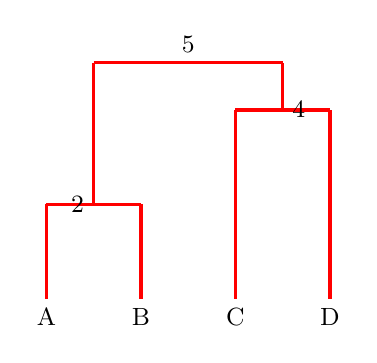
\begin{tikzpicture}[x=1.2cm, y=0.6cm, font=\small]


\foreach \x/\name in {1/A,2/B,3/C,4/D} {
    \node at (\x,0) [below] {\name};
}

\draw<2->   (1,0) -- (1,2);
\draw<2->   (2,0) -- (2,2);
\draw<2->   (1,2) -- (2,2);
\draw<2> [red, very thick] (1,0) -- (1,2) (2,0) -- (2,2) (1,2) -- (2,2);
\node<2-> at (1.5,2) [left] {2};

\draw<3->   (3,0) -- (3,4);
\draw<3->   (4,0) -- (4,4);
\draw<3->   (3,4) -- (4,4);
\draw<3> [red, very thick] (3,0) -- (3,4) (4,0) -- (4,4) (3,4) -- (4,4);
\node<3-> at (3.5,4) [right] {4};


\draw<4->   (1.5,2) -- (1.5,5);
\draw<4->   (3.5,4) -- (3.5,5);
\draw<4->   (1.5,5) -- (3.5,5);
\draw<4> [red, very thick] (1.5,2) -- (1.5,5) (3.5,4) -- (3.5,5) (1.5,5) -- (3.5,5);
\node<4-> at (2.5,5) [above] {5};

\end{tikzpicture}
\end{column}
\end{columns}
\end{frame}


\begin{frame}{Complete Linkage Clustering}
\centering
\textbf{Complete linkage distance:}
\[
D(C_i, C_j) = \max_{x\in C_i,\;y\in C_j} d(x,y)
\]

\vspace{0.3cm}
\begin{columns}[onlytextwidth]
\begin{column}{0.45\textwidth}
\centering
\textbf{Distance Matrix}


\only<1>{
\[
\begin{array}{c|cccc}
    & A & B & C & D \\
\hline
A & 0 & 2 & 6 & 10 \\
B & 2 & 0 & 5 & 9  \\
C & 6 & 5 & 0 & 4  \\
D & 10 & 9 & 4 & 0  \\
\end{array}
\]
}


\only<2>{
\[
\begin{array}{c|cccc}
    & A & B & C & D \\
\hline
A & 0 & \cellcolor{highlight}{2} & 6 & 10 \\
B & \cellcolor{highlight}{2} & 0 & 5 & 9  \\
C & 6 & 5 & 0 & 4  \\
D & 10 & 9 & 4 & 0  \\
\end{array}
\]
}


\only<3>{
\[
\begin{array}{c|ccc}
    & AB & C & D \\
\hline
AB & 0 & \max(6,5)=6 & \max(10,9)=10 \\
C  & 6 & 0 & \cellcolor{highlight}{4} \\
D  & 10 & \cellcolor{highlight}{4} & 0 \\
\end{array}
\]
}


\only<4>{
\[
\begin{array}{c|cc}
    & AB & CD \\
\hline
AB & 0 & \cellcolor{highlight}{\max(6,10)=10} \\
CD & \cellcolor{highlight}{10} & 0 \\
\end{array}
\]
}

\end{column}
\begin{column}{0.4\textwidth}
\centering
\textbf{Dendrogram}
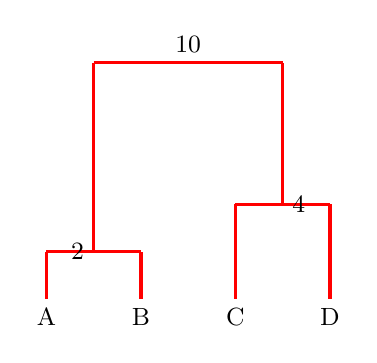
\begin{tikzpicture}[x=1.2cm, y=0.3cm, font=\small]  
\foreach \x/\name in {1/A,2/B,3/C,4/D} {
    \node at (\x,0) [below] {\name};
}


\draw<2->   (1,0) -- (1,2);
\draw<2->   (2,0) -- (2,2);
\draw<2->   (1,2) -- (2,2);
\draw<2> [red, very thick] (1,0) -- (1,2) (2,0) -- (2,2) (1,2) -- (2,2);
\node<2-> at (1.5,2) [left] {2};


\draw<3->   (3,0) -- (3,4);
\draw<3->   (4,0) -- (4,4);
\draw<3->   (3,4) -- (4,4);
\draw<3> [red, very thick] (3,0) -- (3,4) (4,0) -- (4,4) (3,4) -- (4,4);
\node<3-> at (3.5,4) [right] {4};


\draw<4->   (1.5,2) -- (1.5,10);
\draw<4->   (3.5,4) -- (3.5,10);
\draw<4->   (1.5,10) -- (3.5,10);
\draw<4> [red, very thick] (1.5,2) -- (1.5,10) (3.5,4) -- (3.5,10) (1.5,10) -- (3.5,10);
\node<4-> at (2.5,10) [above] {10};

\end{tikzpicture}
\end{column}
\end{columns}
\end{frame}

\begin{frame}{Comparison: Single vs Complete Linkage}
\centering
\textbf{Original Distance Matrix}
\[
\begin{array}{c|cccc}
    & A & B & C & D \\
\hline
A & 0 & 2 & 6 & 10 \\
B & 2 & 0 & 5 & 9  \\
C & 6 & 5 & 0 & 4  \\
D & 10 & 9 & 4 & 0  \\
\end{array}
\]

\vspace{0.3cm}
\begin{columns}[onlytextwidth, T] 
\begin{column}{0.48\textwidth}
\centering
\small\textbf{Single Linkage}\\
$D(C_i,C_j)=\min\limits_{x\in C_i,\;y\in C_j} d(x,y)$

\vspace{0.2cm}
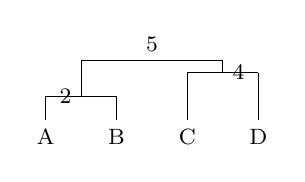
\begin{tikzpicture}[x=0.9cm, y=0.15cm, font=\footnotesize]

\foreach \x/\name in {1/A,2/B,3/C,4/D} {
    \node at (\x,0) [below] {\name};
}

\draw (1,0) -- (1,2);
\draw (2,0) -- (2,2);
\draw (1,2) -- (2,2);
\node at (1.5,2) [left] {2};

\draw (3,0) -- (3,4);
\draw (4,0) -- (4,4);
\draw (3,4) -- (4,4);
\node at (3.5,4) [right] {4};

\draw (1.5,2) -- (1.5,5);
\draw (3.5,4) -- (3.5,5);
\draw (1.5,5) -- (3.5,5);
\node at (2.5,5) [above] {5};
\end{tikzpicture}
\end{column}

\begin{column}{0.48\textwidth}
\centering
\small\textbf{Complete Linkage}\\
$D(C_i,C_j)=\max\limits_{x\in C_i,\;y\in C_j} d(x,y)$

\vspace{0.2cm}
\begin{tikzpicture}[x=0.9cm, y=0.15cm, font=\footnotesize]

\foreach \x/\name in {1/A,2/B,3/C,4/D} {
    \node at (\x,0) [below] {\name};
}

\draw (1,0) -- (1,2);
\draw (2,0) -- (2,2);
\draw (1,2) -- (2,2);
\node at (1.5,2) [left] {2};

\draw (3,0) -- (3,4);
\draw (4,0) -- (4,4);
\draw (3,4) -- (4,4);
\node at (3.5,4) [right] {4};

\draw (1.5,2) -- (1.5,10);
\draw (3.5,4) -- (3.5,10);
\draw (1.5,10) -- (3.5,10);
\node at (2.5,10) [above] {10};
\end{tikzpicture}
\end{column}
\end{columns}

\vspace{0.2cm}
\centering\footnotesize
\emph{Same initial merges (A–B at 2, C–D at 4), but final merge height: 5 (single) vs. 10 (complete).}
\end{frame}

\begin{frame}{Average Linkage Clustering}
\centering
\textbf{Average linkage distance:}
\[
D(C_i, C_j) = \frac{1}{|C_i|\cdot|C_j|} \sum_{x\in C_i} \sum_{y\in C_j} d(x,y)
\]

\vspace{0.2cm}
\begin{columns}[onlytextwidth]
\begin{column}{0.45\textwidth}
\centering
\textbf{Distance Matrix}


\only<1>{
\[
\begin{array}{c|cccc}
    & A & B & C & D \\
\hline
A & 0 & 2 & 6 & 10 \\
B & 2 & 0 & 5 & 9  \\
C & 6 & 5 & 0 & 4  \\
D & 10 & 9 & 4 & 0  \\
\end{array}
\]
}


\only<2>{
\[
\begin{array}{c|cccc}
    & A & B & C & D \\
\hline
A & 0 & \cellcolor{highlight}{2} & 6 & 10 \\
B & \cellcolor{highlight}{2} & 0 & 5 & 9  \\
C & 6 & 5 & 0 & 4  \\
D & 10 & 9 & 4 & 0  \\
\end{array}
\]
}


\only<3>{
\[
\begin{array}{c|ccc}
    & AB & C & D \\
\hline
AB & 0 & \frac{6+5}{2}=5.5 & \frac{10+9}{2}=9.5 \\
C  & 5.5 & 0 & \cellcolor{highlight}{4} \\
D  & 9.5 & \cellcolor{highlight}{4} & 0 \\
\end{array}
\]
}


\only<4>{
\[
\begin{array}{c|cc}
    & AB & CD \\
\hline
AB & 0 & \cellcolor{highlight}{\frac{6+10+5+9}{4}=7.5} \\
CD & \cellcolor{highlight}{7.5} & 0 \\
\end{array}
\]
}

\end{column}
\begin{column}{0.5\textwidth}
\centering
\textbf{Dendrogram}
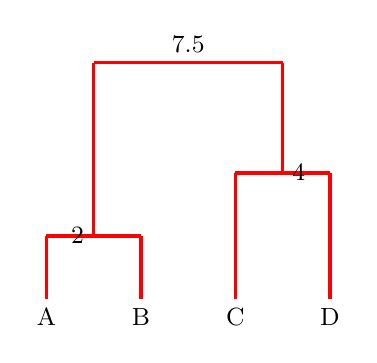
\begin{tikzpicture}[x=1.2cm, y=0.4cm, font=\small]  


\foreach \x/\name in {1/A,2/B,3/C,4/D} {
    \node at (\x,0) [below] {\name};
}


\draw<2->   (1,0) -- (1,2);
\draw<2->   (2,0) -- (2,2);
\draw<2->   (1,2) -- (2,2);
\draw<2> [red, very thick] (1,0) -- (1,2) (2,0) -- (2,2) (1,2) -- (2,2);
\node<2-> at (1.5,2) [left] {2};


\draw<3->   (3,0) -- (3,4);
\draw<3->   (4,0) -- (4,4);
\draw<3->   (3,4) -- (4,4);
\draw<3> [red, very thick] (3,0) -- (3,4) (4,0) -- (4,4) (3,4) -- (4,4);
\node<3-> at (3.5,4) [right] {4};

\draw<4->   (1.5,2) -- (1.5,7.5);
\draw<4->   (3.5,4) -- (3.5,7.5);
\draw<4->   (1.5,7.5) -- (3.5,7.5);
\draw<4> [red, very thick] (1.5,2) -- (1.5,7.5) (3.5,4) -- (3.5,7.5) (1.5,7.5) -- (3.5,7.5);
\node<4-> at (2.5,7.5) [above] {7.5};

\end{tikzpicture}
\end{column}
\end{columns}
\end{frame}

\begin{frame}{Comparison of Linkage Methods}
\centering
\textbf{Distance Matrix}
\[
\begin{array}{c|cccc}
    & A & B & C & D \\
\hline
A & 0 & 2 & 6 & 10 \\
B & 2 & 0 & 5 & 9  \\
C & 6 & 5 & 0 & 4  \\
D & 10 & 9 & 4 & 0  \\
\end{array}
\]

\vspace{0.3cm}
\begin{columns}[onlytextwidth, T]

\begin{column}{0.32\textwidth}
\centering
\small\textbf{Single}\\
$D_{\min}=\min d(x,y)$

\vspace{0.1cm}
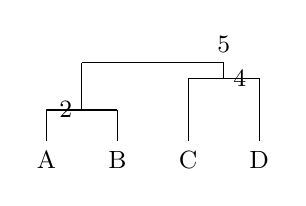
\begin{tikzpicture}[x=0.9cm, y=0.2cm, font=\small]
\foreach \x/\name in {1/A,2/B,3/C,4/D} \node at (\x,0) [below] {\name};
\draw (1,0)--(1,2) (2,0)--(2,2) (1,2)--(2,2) node[left,pos=0.5] {2};
\draw (3,0)--(3,4) (4,0)--(4,4) (3,4)--(4,4) node[right,pos=0.5] {4};
\draw (1.5,2)--(1.5,5) (3.5,4)--(3.5,5) (1.5,5)--(3.5,5) node[above] {5};
\end{tikzpicture}
\end{column}

\begin{column}{0.32\textwidth}
\centering
\small\textbf{Complete}\\
$D_{\max}=\max d(x,y)$

\vspace{0.1cm}
\begin{tikzpicture}[x=0.9cm, y=0.2cm, font=\small]
\foreach \x/\name in {1/A,2/B,3/C,4/D} \node at (\x,0) [below] {\name};
\draw (1,0)--(1,2) (2,0)--(2,2) (1,2)--(2,2) node[left,pos=0.5] {2};
\draw (3,0)--(3,4) (4,0)--(4,4) (3,4)--(4,4) node[right,pos=0.5] {4};
\draw (1.5,2)--(1.5,10) (3.5,4)--(3.5,10) (1.5,10)--(3.5,10) node[above] {10};
\end{tikzpicture}
\end{column}


\begin{column}{0.32\textwidth}
\centering
\small\textbf{Average}\\
$D_{\text{avg}}=\frac{1}{n_i n_j}\sum d$

\vspace{0.1cm}
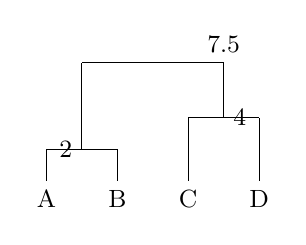
\begin{tikzpicture}[x=0.9cm, y=0.2cm, font=\small]
\foreach \x/\name in {1/A,2/B,3/C,4/D} \node at (\x,0) [below] {\name};
\draw (1,0)--(1,2) (2,0)--(2,2) (1,2)--(2,2) node[left,pos=0.5] {2};
\draw (3,0)--(3,4) (4,0)--(4,4) (3,4)--(4,4) node[right,pos=0.5] {4};
\draw (1.5,2)--(1.5,7.5) (3.5,4)--(3.5,7.5) (1.5,7.5)--(3.5,7.5) node[above] {7.5};
\end{tikzpicture}
\end{column}
\end{columns}

\vspace{0.3cm}
\centering
\emph{Final merge heights: single 5, complete 10, average 7.5.}
\end{frame}



\begin{frame}{The Dendrogram: A Visual Hierarchy}
    \centering
    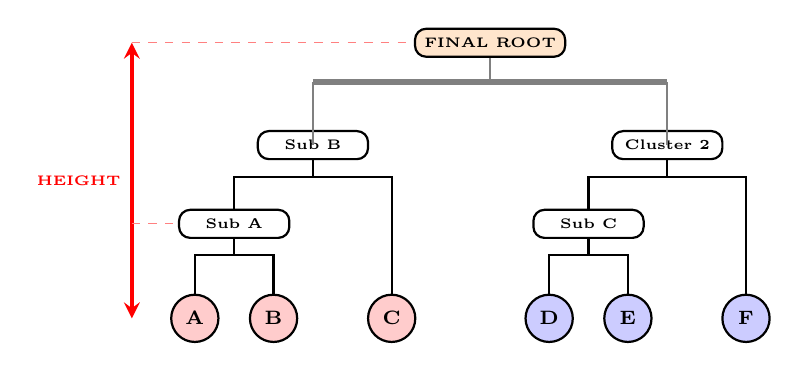
\begin{tikzpicture}[
        leaf/.style={circle, draw, thick, minimum size=0.6cm, font=\scriptsize\bfseries, inner sep=1pt, 
                     fill=red!20},
        branch/.style={rectangle, rounded corners, draw, thick, minimum width=1.4cm, font=\tiny\bfseries, 
                       fill=white},
        line/.style={thick}
    ]

        
        \node[leaf] (A) at (0,0) {A};
        \node[leaf] (B) at (1,0) {B};
        \node[leaf] (C) at (2.5,0) {C};
        \node[leaf, fill=blue!20] (D) at (4.5,0) {D};
        \node[leaf, fill=blue!20] (E) at (5.5,0) {E};
        \node[leaf, fill=blue!20] (F) at (7,0) {F};

        
        \onslide<2->{
            \draw[line] (A) -- (0,0.8) -- (1,0.8) -- (B);
            \node[branch] (SubA) at (0.5, 1.2) {Sub A};
            \draw[line] (0.5,0.8) -- (SubA);
            \draw[line] (D) -- (4.5,0.8) -- (5.5,0.8) -- (E);
            \node[branch] (SubC) at (5, 1.2) {Sub C};
            \draw[line] (5,0.8) -- (SubC);
        }
        
        \onslide<3->{
            \draw[line] (SubA) -- (0.5,1.8) -- (2.5,1.8) -- (C);
            \node[branch] (SubB) at (1.5, 2.2) {Sub B};
            \draw[line] (1.5,1.8) -- (SubB);
            \draw[line] (SubC) -- (5,1.8) -- (7,1.8) -- (F);
            \node[branch] (Clust2) at (6, 2.2) {Cluster 2};
            \draw[line] (6,1.8) -- (Clust2);
        }

        
        \onslide<4->{
            \draw[line, gray, line width=2pt] (1.5,3) -- (6,3);
            \draw[line, gray] (1.5,2.2) -- (1.5,3);
            \draw[line, gray] (6,2.2) -- (6,3);
            \node[branch, fill=orange!20] (Root) at (3.75, 3.5) {FINAL ROOT};
            \draw[line, gray] (3.75,3) -- (Root);
        }

        
        \onslide<5->{
            \draw[<->, >=stealth, red, line width=1.5pt] (-0.8,0) -- (-0.8,3.5) node[midway, left, font=\tiny\bfseries] {HEIGHT};
            \draw[dashed, red!50] (-0.8,1.2) -- (SubA);
            \draw[dashed, red!50] (-0.8,3.5) -- (Root);
        }

    \end{tikzpicture}

    \vspace{0.4cm}
    \begin{description}
        \item<1->[\alert<1>{Leaves:}] Individual data points. 
        \item<2->[\alert<2-3>{Branches:}] Groups formed as we merge similar data.
        \item<4->[\alert<4>{Root:}] The final connection where everything is one.
        \item<5->[\alert<5>{Height:}] The distance at which clusters merge.
    \end{description}
\end{frame}


\begin{frame}{Conclusion}
    \begin{columns}
        \column{0.6\textwidth}
            {\large\bfseries\itshape\color{myblue} Let’s recap the essential concepts:}

            \vspace{0.3cm}
        
            \begin{itemize}
                \item<1-> Hierarchical clustering builds a \textbf{\textcolor{myorange}{tree of clusters}}.
                \item<2-> Two main types: \textbf{Agglomerative} (bottom-up) and \textbf{Divisive} (top-down).
                \item<3-> \textbf{Linkage criteria} define how we measure cluster distance.
                \item<4-> The \textbf{\textcolor{myorange}{dendrogram}} is a powerful visualization tool.
                \item<5-> Widely used in bioinformatics (e.g., phylogenetics), finance (e.g., portfolio analysis), and marketing (e.g., customer segmentation).
            \end{itemize}
        \column{0.4\textwidth}
            \centering
            
\begin{tikzpicture}[scale=0.6]
                
                \draw[myorange, thick] (0,0) -- (0.5,0.6) -- (1.2,0.2) -- (1.8,0.8);
                \filldraw[myorange] (0,0) circle (3pt);
                \filldraw[myorange] (0.5,0.6) circle (3pt);
                \filldraw[myorange] (1.2,0.2) circle (3pt);
                \filldraw[myorange] (1.8,0.8) circle (3pt);
                \node[below, myorange, font=\small] at (0.9,-0.2) {Thank You!};
            \end{tikzpicture}
    \end{columns}
\end{frame}

\end{document}